Two naturally-occurring isotopes of xenon, 134 Xe and 136 Xe, can undergo \bb decay. The latter, having a higher Q value (2458 keV [?,?]), is preferred for \bbonu decay searches. It constitutes only 8.86\% of natural xenon, but the enrichment process is relatively simple and cheap compared to that of other \bb isotopes. The two-neutrino decay mode of \Xe{136} is slow, 2.2 × 10 21 years [?, ?], and hence the experimental requirement for energy resolution is less severe than for other \bb sources. Furthermore, xenon is a suitable detection medium with strong scintillation and ionization primary signals. In its gaseous phase, xenon can provide very good energy resolution, better, in principle, than 0.5\% at the Q value of 136 Xe [?].

The use of xenon gas detectors for \bbonu-decay searches is actually an old idea. The Milano experiment [?], running at LNGS in the late 1980s, made use of a multiwire proportional chamber filled with xenon gas (enriched to 64\% in 136 Xe) at a pressure of 9.5 bars. The detector, with an active volume of 79 litres, contained about 4.4 kg of xenon (32.3 moles of 136 Xe). The detection efficiency, computed with Monte Carlo simulations, was $\simeq$35\%, and the measured energy resolution was 4.5\% FWHM at 2.5 MeV. The background rate in the \bbonu energy window was $\simeq$11 \ckkbby, 4 orders of magnitude worse than current detectors. After accumulating almost 2 kg · yr of exposure, no evidence of any of the \bb decay modes was found in the data. Instead, the following limits to the decay half-lives were reported: \Ttnu > 6.0 × 10 19 years and \Tonu > 2.0 × 10 22 years, both at 90\% CL.

The other pioneer experiment was the Gotthard TPC [?,?], built by a Caltech-PSINeuchâtel collaboration and operated at the St. Gotthard road tunnel (Switzerland) in the 1990s. The key idea of the experiment was the use of the tracking capabilities of the TPC to identify the detected events as signal or background according to their energy deposition pattern (dE/dx), which is unique to a given particle type. For example, Figure ?? (left) shows a typical \bb-candidate event as registered in the Gotthard TPC: a continuos track with extra depositions (blobs) at both ends. Single-track events were selected and scanned visually to classify them as signal or background according to their energy-deposition pattern. The rejection efficiency of single electrons was estimated to be above 98\%.

The detector was filled at a pressure of 5 atm with a 96:4 mixture of xenon gas (enriched to 62.5\% in 136 Xe) and methane, which acted as a quencher increasing the drift velocity and reducing the diffusion of the ionization electrons. The active volume of the detector, of about 180 litres, contained 3.3 kg (24.2 moles) of 136 Xe. The TPC readout system was a classic set of wire grids located behind the anode. The detector had no start-of-event trigger, and hence the absolute longitudinal position of the tracks could not be reconstructed. The achieved energy resolution, 6.5\% FWHM at 2500 keV, was rather modest for xenon. According to simulations, the probability for a \bb event at 2.5 MeV to be completely contained in the active volume of the TPC was 30\%. The measured background rate in the region of interest was about 0.01 \ckkbby, slightly higher than that registered by the Heidelberg-Moscow experiment (§ ??). The dominant background was concluded to be Compton-scattered electrons from natural radioactivity misidentified as twoelectrons events. The following limits to the \bbtnu and \bbonu-decay half-lives were reported: \Ttnu > 3.6 × 10 20 years and \Tonu > 4.4 × 10 23 years at 90\% CL.

The Gotthard TPC demonstrated the effectiveness of tracking in xenon to discriminate signal from background. However, the sensitivity of the experiment was limited by its poor energy resolution. In this chapter we will present the most important physical and operational parameters affecting the energy resolution in gaseous xenon, with some comparisons to the liquid phase. Using arguments based on these experimental factors, we will present a detector design chosen to optimize the energy resolution while keeping the powerful tracking signature.



%%%%%%%nEXO

The nEXO neutrinoless double beta decay experiment is designed to use a time projection chamber and 5000 kg of isotopically enriched liquid xenon to search for the decay in 136Xe. This detector will be based on very successful EXO-200 detector. A single-phase liquid xenon TPC instrumented to read both scintillation and charge. The anti-correlation of these two signals allowed for an energy resolution of 2.89\% FWHM@Qbb \cite{EXO-200:2020wmu}.

This design also provided the capability of a good fidutialization of the events in the detector and, more important, certain capability to separate them by topology. In particular, the separation of single-site and multi-site events [cite] provided a strong background suppression.

The nEXO design aims to build a volume of 5 tonnes of enriched Xe136. The TPC vessel is a right copper cylinder with both inner height and diameter equal to 127.7 cm surrounded by 33,000 kg of HFE-7000, which serves as both thermal bath and radiation shield. A vacuum layer between an inner vessel and an outer vessel of the cryostat provides thermal insulation from an active water shield, referred to as the outer detector. The TPC itself will have 113.3 cm diameter by 118.3 cm drift height, creating a total xenon mass in the drift region of 3648 kg for an active mass of 3281 kg. This design requires 10 ms of electron life-time to guarantee good energy resolution when reading the ionisation signal. This is achieve by a good purification system and a relatively moderate drift field of 400 V/cm. \cite{nEXO:2021ujk}.



%%%%%%
\begin{figure}[t!]
\begin{center}
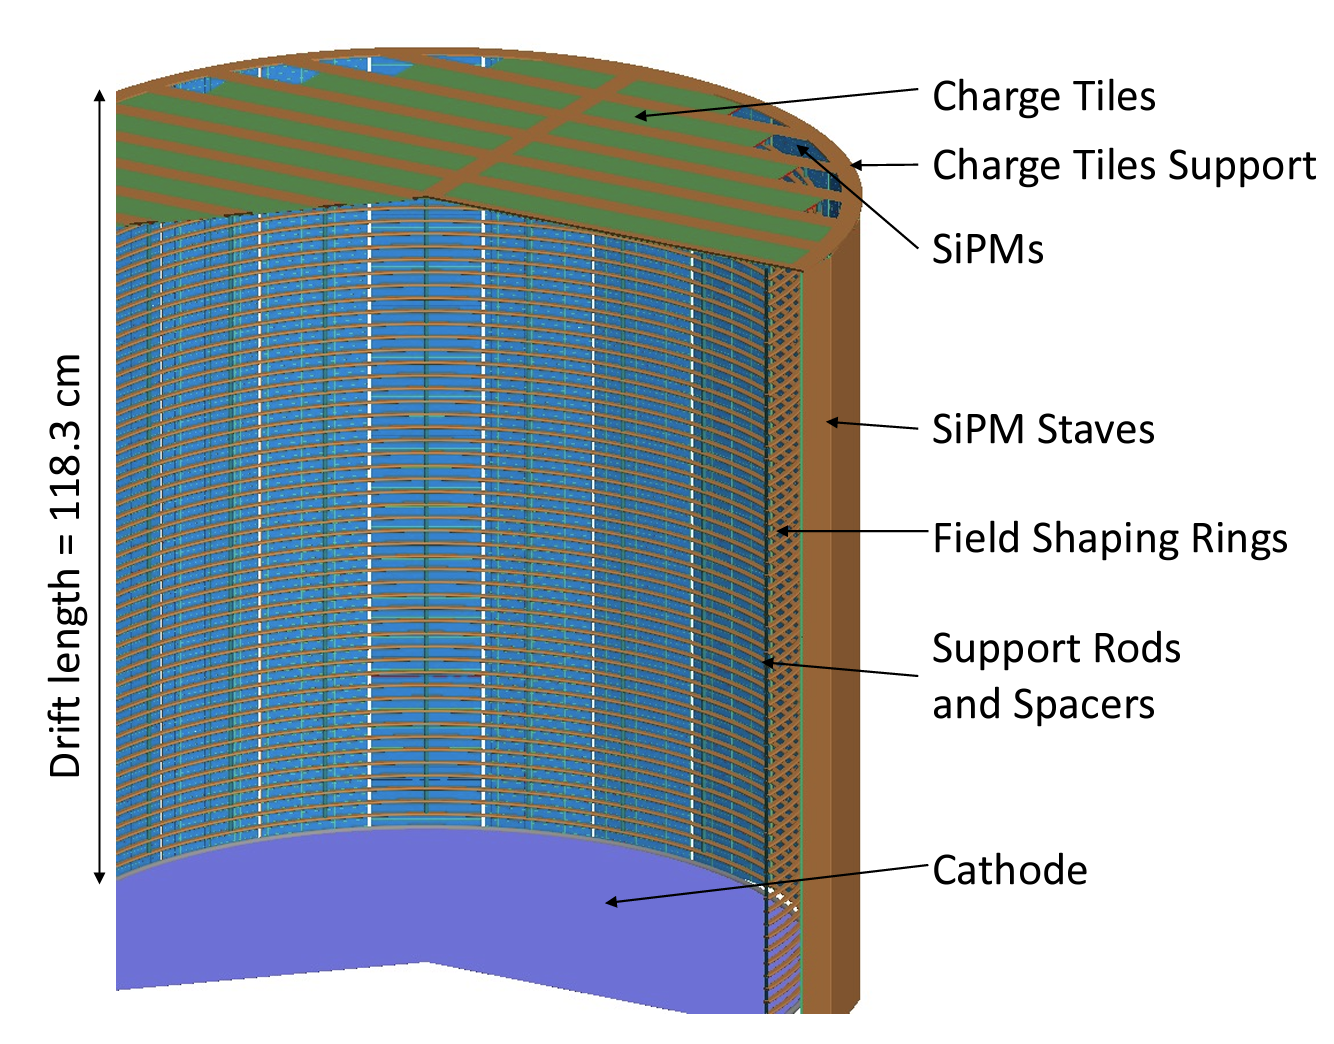
\includegraphics[width=0.475\textwidth]{img/nexo_design}
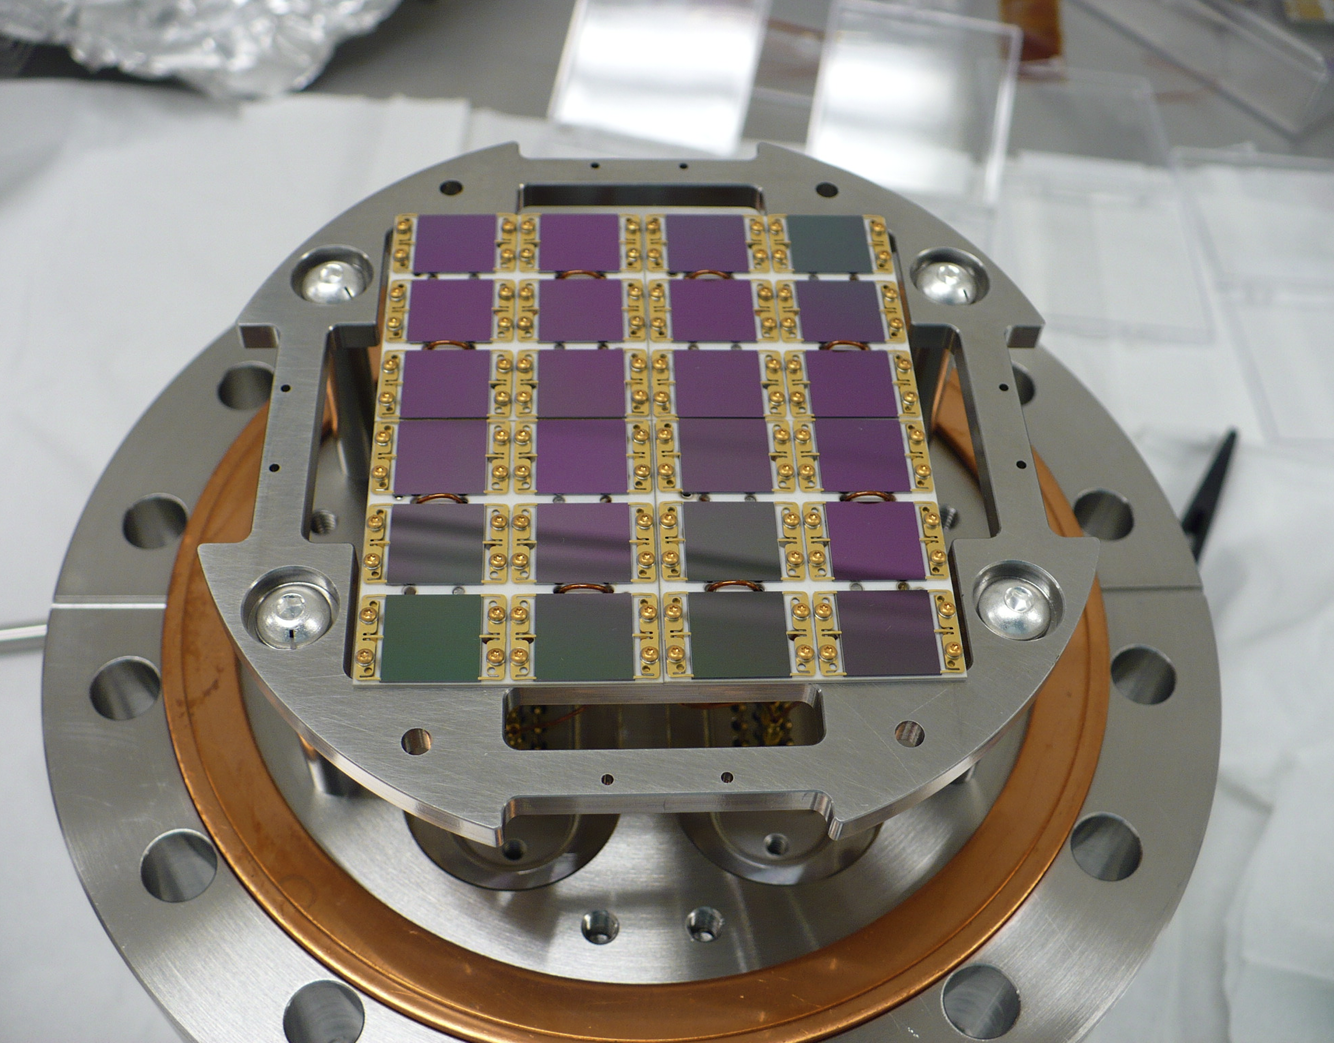
\includegraphics[width=0.475\textwidth]{img/nexo_sipms}
\end{center}
\caption{Left: Close up view of the main components inside the nEXO TPC vessel. Right: Test array of 24 SiPMs used to be used together with charge collection tiles in LXe.Each SiPM is cm$^2$.} \label{fig:nexo}
\end{figure}

Efficient scintillation light collection is an essential requisite for nEXO to attain proper energy resolution and to provide the start time to localize events along the drift field. Actually, in order to reach <2.35\% FWHM energy resolution, the overall optical efficiency must be 3\%  or higher, this is achieved by using SiPMs arrays operated directly in the liquid xenon behind the TPC field shaping rings. The SiPM will have ~1cm$^2$ active area and will be mounted in 24 long staves surrounding the TPC field cage. The necessity of reading as much light as possible has a relevant impact on the TPC design. In particular, the field cage must be as transparent as possible allowing the photons to reach the photsensors region. This affect the geometry of the rings, as they need to be thiner. Also, a coating of vacuum deposited aluminum, protected against oxidation by a layer of MgF2 will make all rings reflective to VUV. In addition, it will allow to remove the traditional PTFE reflective panels used in other liquid xenon TPCs, thus reducing the amount of materials and outgassing inside the detector volume.

One of the main tools the nEXO collaboration proposes to reduce the level of background events is the based on taking advantage of the relatively short attenuation length of $\gamma$-ray at 2.4 MeV energy in LXe, of only 8.7 cm. By selecting a region in the most inner part of the detector they can further reduce the background rate by almost an order of magnitude in the most inner ton of active material. Adding this technique to the energy resolution and topological separation nEXO is predicted to achieve a background rate of 3.6 × 10$^{-4}$ cts/(FWHM·kg·y) in the inner 2000 kg of LXe. 

With this level of background nEXO aims to reach a sensitivity of 9.2 × 10$^{27}$ yrs at 90\% C.L. after 10 years of operation and, an expected 3 sigma discovery potential of 5.7 × 
10$^{27}$ yrs \cite{nexocprecdr}. However, in a recent document \cite{nEXO:2021ujk} the nEXO Collaboration claims for an improved design and understanding of the nEXO design, together with the development of a \bbonu\ DNN discriminator that pushes the background index to 
b=7×10$^{-5}$ cts/(FWHM·kg·yr) obtaining a half-life sensitivity of 1.35×10$^{28}$ 
yr at 90\% C.L.

NEXT is an international effort dedicated to the search for \bbonu\ decay in \Xe{136} using high-pressure xenon gas time projection chambers (HPXeTPC) with amplification of the ionization signal by electroluminescence (EL). This detector technology takes advantage of the inherently low fluctuations in the production of ionization pairs (i.e., small Fano factor) in xenon gas to achieve an energy resolution significantly better than that of other \Xe{136}-based double-beta decay experiments \cite{Nygren:2009zz}. Moreover, the tracks left in gaseous xenon by \bbonu\ events have distinct features that can be used for background rejection. 

Over the last decade, the NEXT Collaboration has proven the performance of the HPXeTPC technology in the key parameters required for the observation of \bbonu\ decay. The NEXT concept was initially tested in small, surface-operated detectors \cite{Alvarez:2012kua, Alvarez:2012xda, Alvarez:2013gxa, Lorca:2014sra, Ferrario:2015kta}. This phase was followed by the underground operation at the LSC of NEXT-{\sc White} \cite{Monrabal:2018xlr}, an asymmetric, radiopure HPXeTPC containing approximately 5~kg of xenon at 10~bar pressure. The results obtained with NEXT-{\sc White} include the development of a procedure to calibrate the detector using \Kr{83m} decays \cite{Martinez-Lema:2018ibw}, measurement of an energy resolution at 2.5~MeV better than 1\% FWHM \cite{Renner:2018ttw, Renner:2019pfe}, demonstration of robust discrimination between single-electron and double-electron tracks \cite{Ferrario:2019kwg}, and measurement of the radiogenic background, validating the accuracy of our background model \cite{Novella:2018ewv,Novella:2019cne}.

The NEXT-100 detector \cite{Alvarez:2012sma}, scheduled to start operation in 2023, constitutes the third phase of the program. It is an asymmetric HPXeTPC containing about 100~kg of xenon (enriched at $\sim$90\% in \Xe{136}) at 15~bar. NEXT-100 will reach a sensitivity of about $6\times10^{25}$~year after a run of 3 effective years, for a predicted background rate of at most $4\times10^{-4}$ \ckky.

A scaled-up version of this technology with about 1 tonne of enriched xenon could reach in less than 5 years of operation a sensitivity to the half-life of \bbonu\ decay better than $10^{27}$~years, improving the current limits by at least one order of magnitude. The NEXT Collaboration is also pursuing a more radical approach to a tonne-scale experiment based on the efficient detection of the Ba++ ion produced in the double-beta decay of Xe-136 using single-molecule fluorescence imaging (SMFI).